% Chapter Comecocos Online Multiplayer
\chapter{Comecocos Online Multiplayer}
\section{Enunciado}
En la comunidad de internet han aumentado el desarrollo de aplicaciones en tiempo real entre distintos usuarios que se encuentran en diferentes partes del mundo.
Esta segunda practica es una extensión de la primera ya que ahora el juego se va a ser multijugador online por medio de interfaz Web.
\begin{figure}[!h]
\begin{center}
  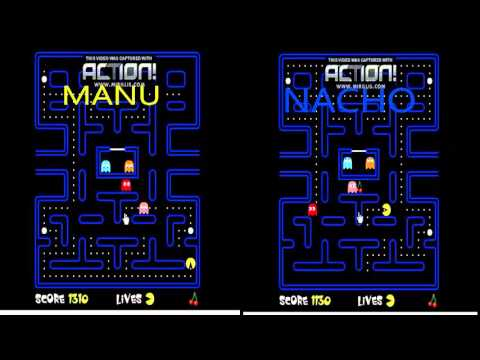
\includegraphics[width=0.5\linewidth]{Figures/introMultiplayer}
	\decoRule
	\caption[Ejemplo Aspecto multijugador Pacman]{Ejemplo Aspecto multijugador Pacman.}
\label{fig:Pacman_Intro2}
\end{center}
\end{figure}
\subsection{Requisitos}
El comportamiento del juego sera el desarrollado en la primera practica pero sera necesario organizarlo de tal forma que el cliente se encargue de ciertas tareas y el servidor de otras con el objetivo de intercambiar información por medio de WebSockets, a continuación se explica en detalle cada una.
\begin{enumerate}
\item\textbf{Cliente}
\begin{itemize}
\item  Conexión WebSockets con el servidor.
\item  Dibujar el escenario del juego,fantasmas,jugadores e información de la partida.
\item  Gestión del movimiento del personaje por medio de los eventos del teclado.
\end{itemize}
\item\textbf{Servidor}
\begin{itemize}
\item Entregar el fichero que contiene la aplicación.
\item Conexión WebSockets con los clientes.
\item Creación de un modulo que contenga los valores iniciales del juego como los cocos,obstáculo entre otros y un objeto de tipo \textbf{Player} que contenga la posición del usuario y del fantasma correspondiente.
\item Se encargara de la lógica de los fantasmas aplicada en la primera practica. Hay que remarcar que en esta versión solo existe un fantasma por usuario.
\item Por medio de la conexión WebSockets gestiona la entrada en sala,inicio del juego y la actualización de los distintos elementos del juego.
\end{itemize}
\end{enumerate}
\subsection{Tecnologías necesarias}
  \begin{enumerate}
    \item WebSockets.
    \item JavaScript.
    \item NodeJS.
  \end{enumerate}
\section{Desarrollo}
El desarrollo se separa en cliente y servidor, aunque existen funciones \footnote{Apéndice A} que no explicamos a fondo ya que son las mismas que las de la primera practica o son auxiliares.
\section{Servidor}
El servidor de la aplicación lo desarrollamos con NodeJS por lo que se importa las librerías \textbf{node-static} y \textbf{http} para la creación del servidor.
\\Con esto el servidor entrega el fichero inicial a los usuarios que se conecten pero queda importar la librería \textbf{socket.io} para crear la conexión WebSockets en el momento de recibir una petición.
\begin{lstlisting}[
caption=Definición del servidor.]
 var static = require('node-static');
 var http = require('http');
 var file = new(static.Server)();
 var app = http.createServer(function (req, res) {
  file.serve(req, res);
  console.log('Server listinig 8181');
 }).listen(8181);
 /*  inst. socket.io  */
 var io = require('socket.io').listen(app);
\end{lstlisting}
La imagen \ref{fig:EjecucionServer} muestra la conexión de un cliente al servidor y el inicio de la conexión WebSockets.
\begin{figure}[!h]
\begin{center}
  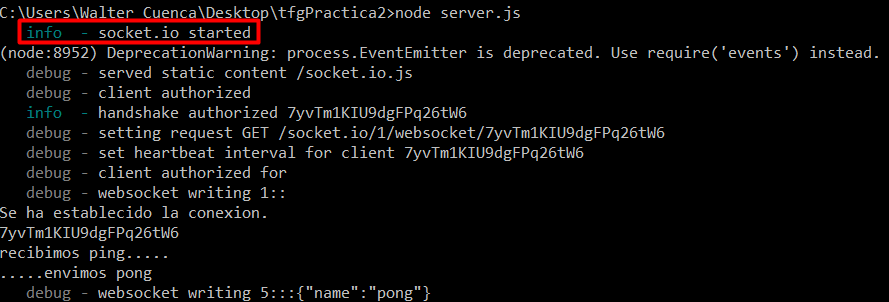
\includegraphics[width=0.7\linewidth]{Figures/Init_Server}
	\decoRule
	\caption[Ejecución del servidor]{Ejecución del servidor.}
\label{fig:EjecucionServer}
\end{center}
\end{figure}
\subsection{Modulo Game}
Se crea el modulo \textbf{CoreServer.js} en NodeJs para separar la lógica y las variables que definen los elementos del juego.Este modulo primero define las variables que tienen relación con el aspecto del juego como son los obstáculos, cocos y propiedades del juego.
\begin{lstlisting}[
caption=Definición variables del Obj.Game]
 var map = [...
 ];
 /* Jugadores */
 var player1 = {'x':5,'y':15,'typePacman':1,numPasos:0};
 var player2 = {'x':11,'y':3,'typePacman':2,numPasos:0};
 /*  */
 var list_user=[];
 var name_room = 'hallGame';

 /* Cronometro */
 var seconds = 0;
 var min = 0;
 var horas = 0;
 var time = '00'+':'+'00'+':'+'00';
 var _timer;
 var list_cocos = [
 ];
 var list_obstaculos = [
 ];
 var properGame={
	'wCuad':40,
	'hCuad':40, 
	'nColum':18,
	'nFila':19,
 }
 var shape_1 = [....
 ];
 var shape_2 = [....
 ];
\end{lstlisting}
Por otro lado define el objeto \textbf{Player} para representar a cada jugador. El objeto contiene la posición y pasos del personaje e incluye la posición y lista de nodos del fantasma correspondiente.
\begin{lstlisting}[
caption=Definición Player Obj.Game]
 function Player(x,y,typePacman,xGhost,yGhost){
  this.info= {'x':x,
   'y':y,
   'typePacman':typePacman,
   'numPasos':0,
   'fantasma': {'x':xGhost,
     'y':yGhost,
    },
  };
  this.path = [];
}
\end{lstlisting}
Para que el contenido del modulo sea accesible desde el servidor es necesario declarar los elementos como \textbf{module.exports}.
\begin{lstlisting}[
caption=Export elementos del Obj.Game]
 module.exports = {
  'map':map,
  'shape_1':shape_1,
  'shape_2':shape_2,
  'properGame':properGame,
  'list_obstaculos':list_obstaculos,
  'list_cocos':list_cocos,
  'name_room':name_room,
  '_timer;':_timer,
  'seconds':seconds,
  'min':min,
  'horas':horas,
  'time':time,
  'Player':Player
 }
\end{lstlisting}
Tras esto volvemos al fichero \textbf{server.js} donde se declara el acceso al modulo a través de la variable \textbf{Game}. A partir de ella creamos la instancia de los jugadores y calculamos la lista de nodos de su correspondiente fantasma por medio de la función auxiliar \textbf{CreatePath()}.
\begin{lstlisting}[
caption=Instancia Jugadores del Servidor.]
 var Game = requiere('./ghost.js')
	
 /* posiciones iniciales */
 var player1 = new Game.Player(5,15,1,1,1);
 var player2 = new Game.Player(14,15,2,18,1);
 player1.path = CreatePath(player1.info,player1.info.fantasma);
 player2.path = CreatePath(player2.info,player2.info.fantasma);
\end{lstlisting}
\subsection{Lógica del Servidor}
Hasta este momento solo se ha definido los elementos del juego pero no se ha visto como el servidor gestiona cada uno de los estados del juego hasta que este finaliza.
\\Aquí es donde \textbf{WebSockets} interviene por medio de la librería \textbf{socket.io}, ya que permite al servidor gestionar los mensajes que recibirá. A continuación, se explican los tipos de mensajes y su tratamiento.
\subsubsection*{Sala de juego}
Definimos el evento \textbf{stablish\_connection} que recibe el nombre del usuario para validar la entrada a la sala.
\\Primero comprueba el numero de usuario en la sala ya que esta restringido a dos. Si aun no esta completa comprueba que el nombre del usuario no exista por medio de la función \textbf{seekUser(name)}. Si existe el nombre envía un mensaje \textbf{reject\_name} en caso contrario envía un mensaje \textbf{CreateConnection} con el id de la conexión y la lista de usuario dentro de la sala.
\\Finaliza vinculando la conexión del usuario a la sala del juego y actualizando la lista de usuarios.
\begin{lstlisting}[
caption=Definición evento stablish\_connection]
 socket.on('stablish_connection',function(name){
  var numClients = io.sockets.clients(Game.name_room).length;
  var existeName = seekUser(name);
  if(existeName){
   var txt = 'El nombre ya existe en esta sala';
   socket.emit('reject_name',txt);
  }else{
   socket.emit('CreateConnection',socket.id,list_user); 
   socket.username = name;
   socket.room = Game.name_room;
   socket.join(Game.name_room);
   if(list_user.length == 0){
    var user = {'user':name,'room':Game.name_room,'id':socket.id,'posGame':player1.info,'pos':1,'score':0};
   }else{
    var user = {'user':name,'room':Game.name_room,'id':socket.id,'posGame':player2.info,'pos':2,'score':0};
   }
   list_user.push(user);
   socket.broadcast.to(Game.name_room).emit('New_Joined',socket.id);
  }
 });
\end{lstlisting}
La figura \ref{fig:Init_Room_1} muestra la conexiona del primer jugador mientras la figura \ref{fig:Init_Room_2} trata la del segundo jugador.
\begin{figure}[!h]
\begin{center}
  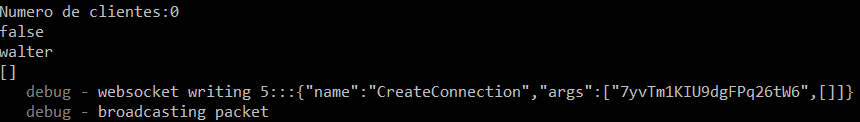
\includegraphics[width=0.9\linewidth]{Figures/Init_Room}
	\decoRule
	\caption[ServidorSeñalizacion]{Petición sala 1ª jugador.}
\label{fig:Init_Room_1}
\end{center}
\end{figure}
\begin{figure}[!h]
\begin{center}
  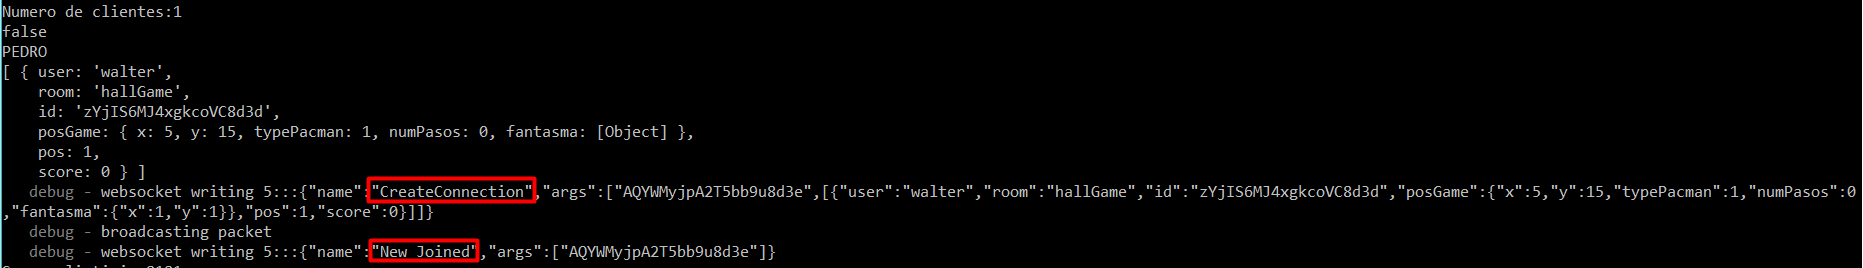
\includegraphics[width=0.9\linewidth]{Figures/Init_Room_2}
	\decoRule
	\caption[ServidorSeñalizacion]{Petición sala 2º jugador.}
\label{fig:Init_Room_2}
\end{center}
\end{figure}
\subsubsection{Petición de partida}
La petición y respuesta a la creación de una partida la realizan los usuarios por lo que el servidor en este caso sera transparente para ellos. Por ello definimos el evento \textbf{message} que encamina los mensajes entre los usuarios por medio del valor \textbf{idDestino}.
\begin{lstlisting}[
caption=Definición evento message.]
 socket.on('message',function(message){
  io.sockets.socket(message.idDestino).emit('message', message);
 });
\end{lstlisting}
En la figura \ref{fig:ServerMessage} se muestra como el servidor encamina los mensajes entre los usuarios.
\begin{figure}[!h]
\begin{center}
  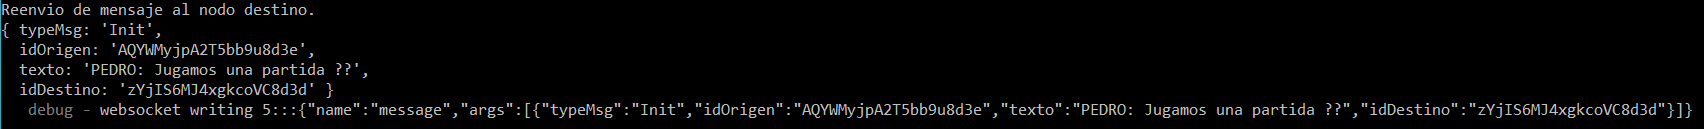
\includegraphics[width=0.9\linewidth]{Figures/Server_Message}
	\decoRule
	\caption[Petición de partida usuario.]{Petición de partida usuario.}
\label{fig:ServerMessage}
\end{center}
\end{figure}
\begin{figure}[!h]
\begin{center}
  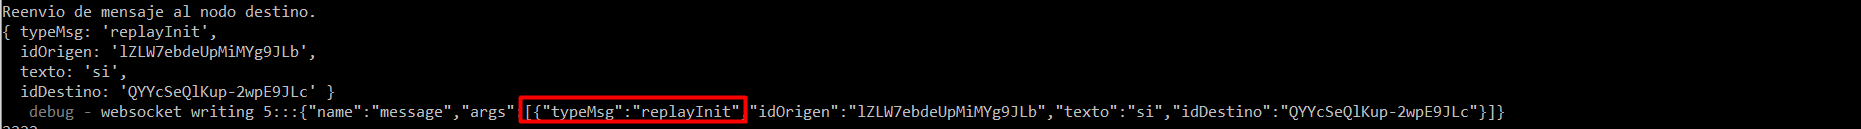
\includegraphics[width=0.9\linewidth]{Figures/Server_Message_2}
	\decoRule
	\caption[Respuesta de partida usuario.]{Respuesta de partida usuario.}
\label{fig:ServerMessage}
\end{center}
\end{figure}
\subsubsection{Elementos del juego}
Tras haber acordado jugar una partida ambos jugadores se define el evento \textbf{Request\_ElementGame} para enviar los parámetros iniciales del juego.
\\Obtiene la información de los jugadores utilizando la función \textbf{getInfoUser(id)} pasándole cada uno de los identificadores.
\\Con la información anterior y las características del escenario crea la variable \textbf{elements} que se envía dentro del mensaje \textbf{Response\_ElementGame}.
\begin{lstlisting}[
caption=Definicion del evento Request\_ElementGame]
 socket.on('Request_ElementGame',function(otherId){
  var myInfo = getInfoUser(socket.id);
  var counterInfo = getInfoUser(otherId);
  var element = {
   'shape_1':Game.shape_1,
   'shape_2':Game.shape_2,
   'cocos':Game.list_cocos,
   'obstaculos':Game.list_obstaculos,
   'properGame':Game.properGame,
   'myInfo':myInfo,
   'counterInfo':counterInfo
  }
  socket.emit('Response_ElementGame',element);
 });
\end{lstlisting}
La figura \ref{fig:Response_elementGame} muestra el envió de la información a los jugadores.
\begin{figure}[!h]
\begin{center}
  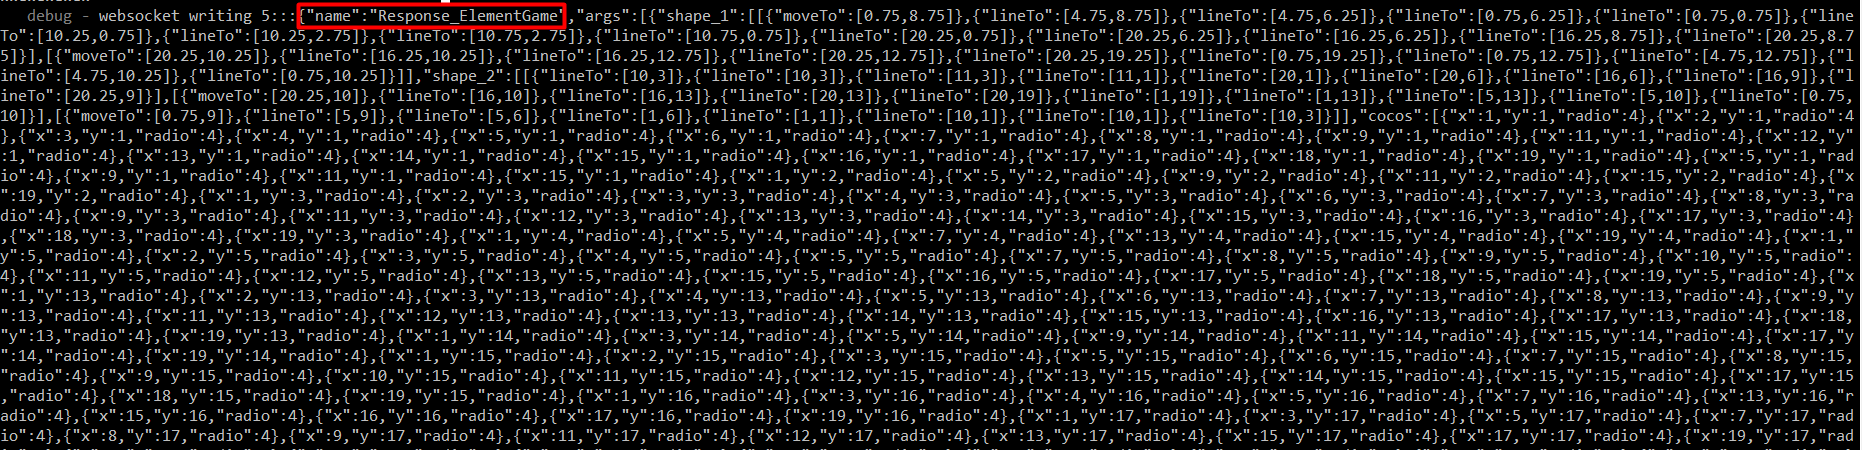
\includegraphics[width=0.9\linewidth]{Figures/Response_elementGame}
	\decoRule
	\caption[Envió elementos del juego.]{Envió elementos del juego.}
\label{fig:Response_elementGame}
\end{center}
\end{figure}
\subsubsection{Inicio del juego}
Para iniciar la partida definimos el evento \textbf{Finish\_InitFrame}. Se encarga de validar que la petición de inicio de partida este solicitada por los dos jugadores para enviar el mensaje \textbf{ReadyGame} a los clientes.
\\En este punto se establece el bucle de actualización del juego por parte del servidor a los cliente por medio del evento timer \textbf{setInterval(UpdateGhost,800)}.
\begin{lstlisting}[
caption=Definición del evento Finish\_InitFrame]
 socket.on('Finish_InitFrame',function(){
  cooordiar +=1;
  if(cooordiar == 2){
   io.sockets.in(Game.name_room).emit('ReadyGame');
   setTimeout(function(){
    Game._timer = setInterval(UpdateGhost,800);
    CronoTime();
   },3000)
  }
 });
\end{lstlisting}
La función \textbf{UpdateGhost} es la parte mas importante de la lógica del servidor ya que se encarga de actualizar la posición de cada fantasma y obtener la puntuación de cada usuario para enviar un mensaje \textbf{NewPos\_Ghost}.
\\También comprueba si alguno de los usuarios a colisionado con el fantasma lo que provoca que se envié el mensaje \textbf{State\_Game} a los usuarios.
\begin{lstlisting}[
caption=Definición de la función UpdateGhost.]
 function UpdateGhost(){
  var elementsGame = [];
  /*  */
  var hitGhost1 = playerHitGhost(player1); //true o false
  var hitGhost2 = playerHitGhost(player2); // true o false
  if (!hitGhost1 && !hitGhost2){
   var coordGhost={'x':player1.path[0].x,'y':player1.path[0].y};
  	setGhost_User(list_user[0].id,coordGhost);
  	coordGhost={'x':player2.path[0].x,'y':player2.path[0].y};
  	setGhost_User(list_user[1].id,coordGhost);
  	elementsGame.push({'id':list_user[0].id,'x':player1.path[0].x,'y':player1.path[0].y,'score':list_user[0].score});
  	player1.path.splice(0,1);
  	elementsGame.push({'id':list_user[1].id,'x':player2.path[0].x,'y':player2.path[0].y,'score':list_user[1].score}});
  	player2.path.splice(0,1);
  	io.sockets.in(Game.name_room).emit('NewPos_Ghost',fantasmas,Game.time,scores);
  }

  if (hitGhost1 || hitGhost2){
  	var msgPlayer1 = (hitGhost1 === true ) ? 'KO' : 'OK';
  	var msgPlayer2 = (hitGhost2 === true ) ? 'KO' : 'OK';
  	io.sockets.socket(list_user[0].id).emit('State_Game', msgPlayer1);
  	io.sockets.socket(list_user[1].id).emit('State_Game', msgPlayer2);
  	clearInterval(Game._timer);
  }  
}
\end{lstlisting}
La figura \ref{fig:Update_GhostPosition} muestra el envió de la información actualizada del juego a los jugadores.
\begin{figure}[!h]
\begin{center}
   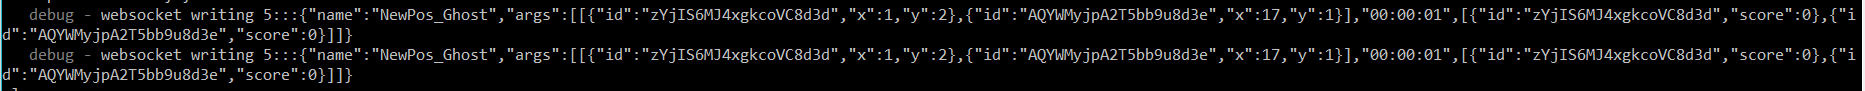
\includegraphics[width=0.9\linewidth]{Figures/Update_GhostPosition}
	\decoRule
	\caption[Envio actualización del juego.]{Envió actualización del juego.}
\label{fig:Update_GhostPosition}
\end{center}
\end{figure}
\subsubsection{Actualización elementos del juego}
El movimiento del personaje de cada usuario es notificado al servidor por lo que se define el evento \textbf{UpdatePosition\_Player}. Con la nueva posición actualiza la posición del personaje correspondiente por medio de la función \textbf{setPosition\_User}.
\\Ademas, evalúa el numero de pasos dado por el personaje ya que si el valor es 1 o -1 indica que se ha movido a una nueva casilla del mapa de juego y es necesario actualizar la lista de nodos que contiene la variable \textbf{path}.
\\Finalmente envía el mensaje \textbf{NewPos\_Counter} con la nueva posición al usuario contrario.
\begin{lstlisting}[
caption=Definición del evento UpdatePosition\_Player.]
 socket.on('UpdatePosition_Player',function(newPosition){
  setPosition_User(socket.id,newPosition);
  if(newPosition.numPasos == 1 || newPosition.numPasos == -1){
   for (var i = 0; i < list_user.length; i++) {
    var user = list_user[i];
    if(user.id == socket.id){
     var myInfo = getInfoUser(socket.id)
     if (user.pos == 1) {
      player1.path = CreatePath(myInfo,myInfo.fantasma);
     }else{
      player2.path = CreatePath(myInfo,myInfo.fantasma);
     }
    }
   }
  }
  socket.broadcast.to(Game.name_room).emit('NewPos_Counter',newPosition);
 });
\end{lstlisting}
La figura \ref{fig:Server_NewPos_Counter} muestra el envió de la nueva posición al usuario contrario.
\begin{figure}[!h]
\begin{center}
   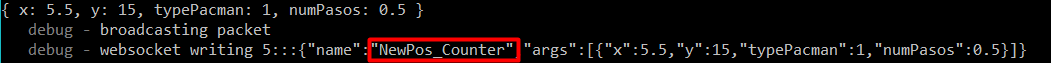
\includegraphics[width=0.9\linewidth]{Figures/Server_NewPos_Counter}
	\decoRule
	\caption[Envio actualización del juego.]{Envió nueva posición usuario.}
\label{fig:Server_NewPos_Counter}
\end{center}
\end{figure}
\\El movimiento del personaje provoca interacción con los cocos por lo que definimos el evento \textbf{UpdateCocos\_Player} que se encarga de eliminar el elemento de la lista de cocos y reenviar la información al otro jugador por medio del mensaje \textbf{UpdateCocos\_Player}.
\\Por ultimo, comprueba si no existen mas cocos en el juego ya que si esto ocurre se envía el mensaje \textbf{GameWinner} a los jugadores informando quien a ganado.
\begin{lstlisting}[
caption=Definición del evento UpdateCocos.]
 socket.on('UpdateCocos',function(cocoPosition){
  Game.list_cocos.splice(cocoPosition,1);
  socket.broadcast.to(Game.name_room).emit('UpdateCocos_Player',cocoPosition);
  setScore_User(socket.id,4);
  if(Game.list_cocos.length == 0){
   ganador = gameFinish();
   io.sockets.in(Game.name_room).emit('GameWinner',ganador);
  }
 });
\end{lstlisting}
La figura \ref{fig:Server_NewPos_Counter} muestra el envió del coco comido por un usuario al contrario.
\begin{figure}[!h]
\begin{center}
   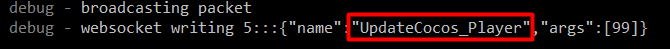
\includegraphics[width=0.9\linewidth]{Figures/Server_UpdateCoco}
	\decoRule
	\caption[Envió coco comido al usuario.]{Envió coco comido al usuario.}
\label{fig:Update_ElementsPosition}
\end{center}
\end{figure}
\section{Cliente}
Los jugadores que conectan a la url \textbf{http://localhost:8181/} en la que se encuentra el servidor que entrega el fichero \textbf{index.html} \footnote{Apéndice A} al navegador estableciendo la conexión WebSockets con el servidor.
\begin{figure}[!h]
\begin{center}
   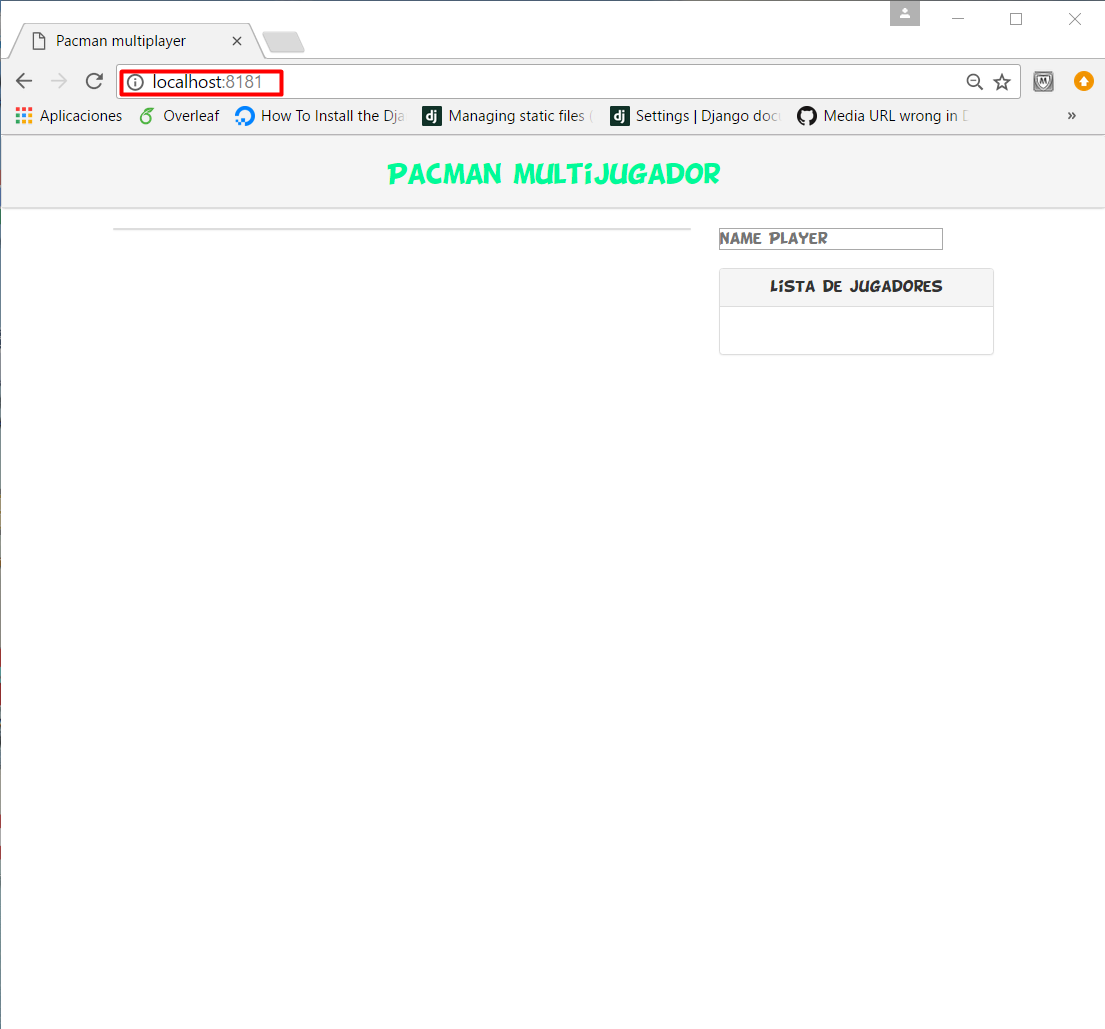
\includegraphics[width=0.4\linewidth]{Figures/Init_Client}
	\decoRule
	\caption[Pagina Inicio Pacman-Online]{Pagina Inicio Pacman-Online.}
\label{fig:Init_Client}
\end{center}
\end{figure}
\subsection{Lógica de comunicación}
Ahora se muestra los distintos mensajes y eventos definimos en el cliente para establecer la comunicación.
\subsubsection*{Sala de juego}
El usuario introduce el nombre en el \textbf{input} de la pagina, provocando que se envíe un mensaje \textbf{stablish\_connection} con el nombre para validar que no existe en la sala.
\begin{lstlisting}[
caption=Envió mensaje stablish\_connection.]
 function sendConnection(){
  socket.emit('stablish_connection',$('#player').val());
  $('#player').attr('disabled',true);
 }
\end{lstlisting}
Se genera el evento \textbf{Reject\_name} para tratar la respuesta al mensaje en caso de que el nombre no sea valido.
\begin{lstlisting}[
caption=Definición evento reject\_name.]
 socket.on('reject_name',function(info){
 $('#player').attr('disabled',false);
});
\end{lstlisting}
Por ultimo, se crea el evento \textbf{CreateConnection} para tratar en caso de ser afirmativa la respuesta al mensaje. Recibe el \textbf{id} de la conexión con el que se crea la instancia del objeto \textbf{Player} en la variable \textbf{myPacman} y la lista de usuario. 
\begin{lstlisting}[
caption=Definición evento CreateConnection.]
 socket.on('CreateConnection',function(id,listUser){
  listplayers = listUser;
  myPacman = new Player(id);
  for (var i = 0; i < listUser.length; i++) {
   var player = listUser[i];
   $('.list-group').append('<li id=user_'+i+' class=list-group-item>'+player.user+'</li>');
   $('#user_'+i).click(function(){requestGame(this)});
  }	
 });
\end{lstlisting}
La figura \ref{fig:Init_Client1_Room} muestra la petición de sala del primer usuario mientras que la figura \ref{fig:Init_Client_2_Room} del segundo.
\begin{figure}[!h]
\begin{center}
  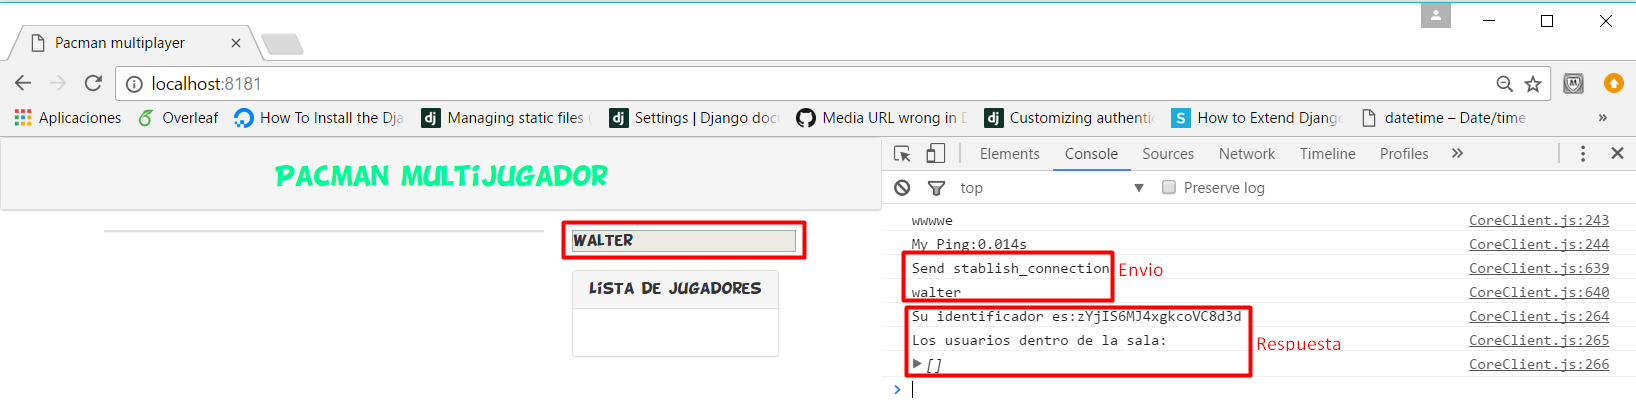
\includegraphics[width=0.6\linewidth]{Figures/Init_Client1_Room}
	\decoRule
	\caption[Petición/Respuesta sala 1ª jugador.]{Petición/Respuesta sala 1ª jugador.}
\label{fig:Init_Client1_Room}
\end{center}
\end{figure}

\begin{figure}[!h]
\begin{center}
   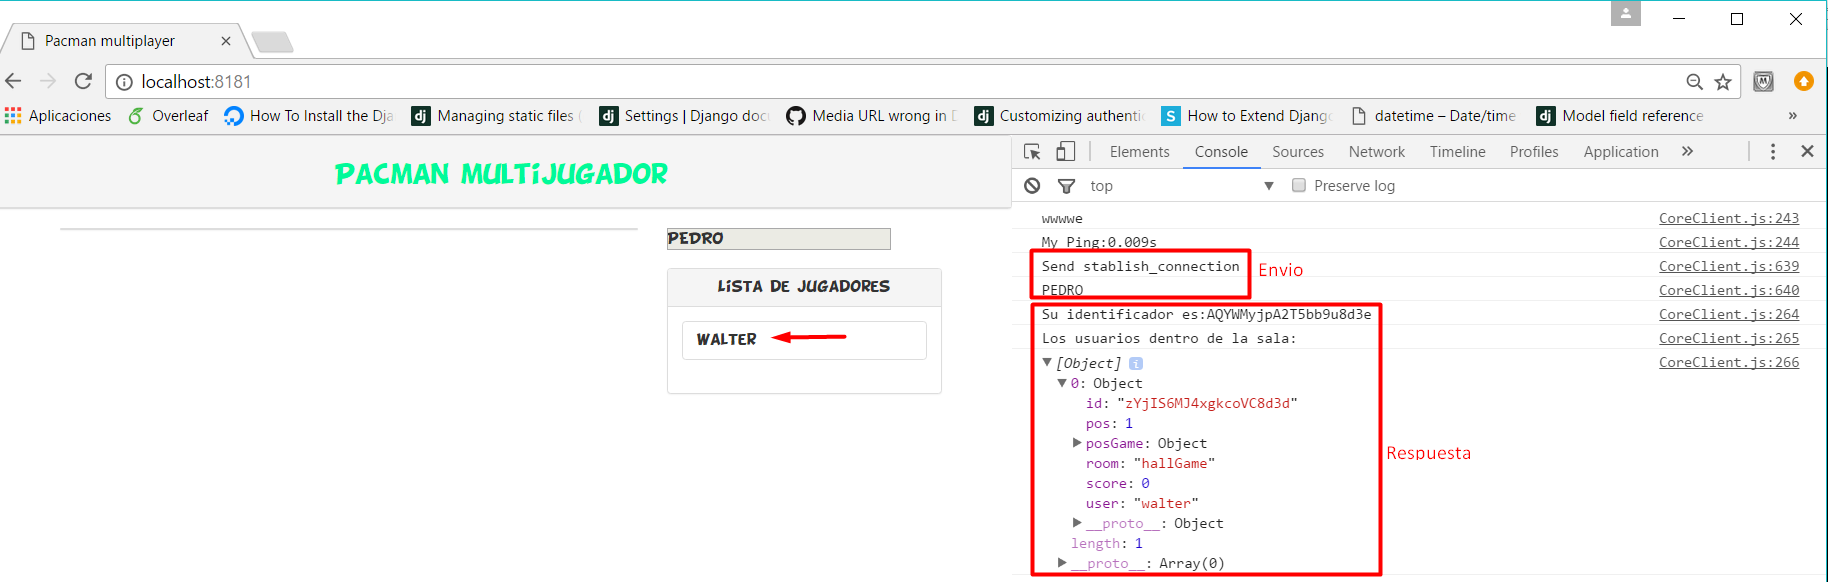
\includegraphics[width=0.6\linewidth]{Figures/Init_Client_2_Room}
	\decoRule
	\caption[Petición/Respuesta sala 2ª jugador.]{Petición/Respuesta sala 2ª jugador.}
\label{fig:Init_Client_2_Room}
\end{center}
\end{figure}
\subsubsection*{Petición de Partida}
Tras entrar en la sala los usuarios pueden realizar una petición de partida a los usuarios existentes. Al seleccionar un nombre de la lista se active la función \textbf{RequestGame(this)}.
\\Esta función se encarga de obtener el id de la conexión del cliente seleccionado por medio de la función \textbf{SeekUser(name)} y genera un mensaje \textbf{message} cuyo cuerpo contiene el \textbf{id\_origen}, \textbf{id\_destino} , el texto de la petición y como subtipo de mensaje \textbf{Init}.
\begin{lstlisting}[
caption=Definición función requestGame.]
 function requestGame(elemento){
  var text=$('#player').val()+': Jugamos una partida ??';
  var destino = seekID($(elemento).text());
  var message = {
   'typeMsg':'Init',
   'idOrigen':myPacman.id,
   'texto':text,
   'idDestino':destino
  }
  socket.emit('message',message)
  $('li').off('click');
 }
\end{lstlisting}
La imagen \ref{fig:Client2_Peti_Game} muestra la petición de partida de un jugador a otro.
\begin{figure}[!h]
\begin{center}
   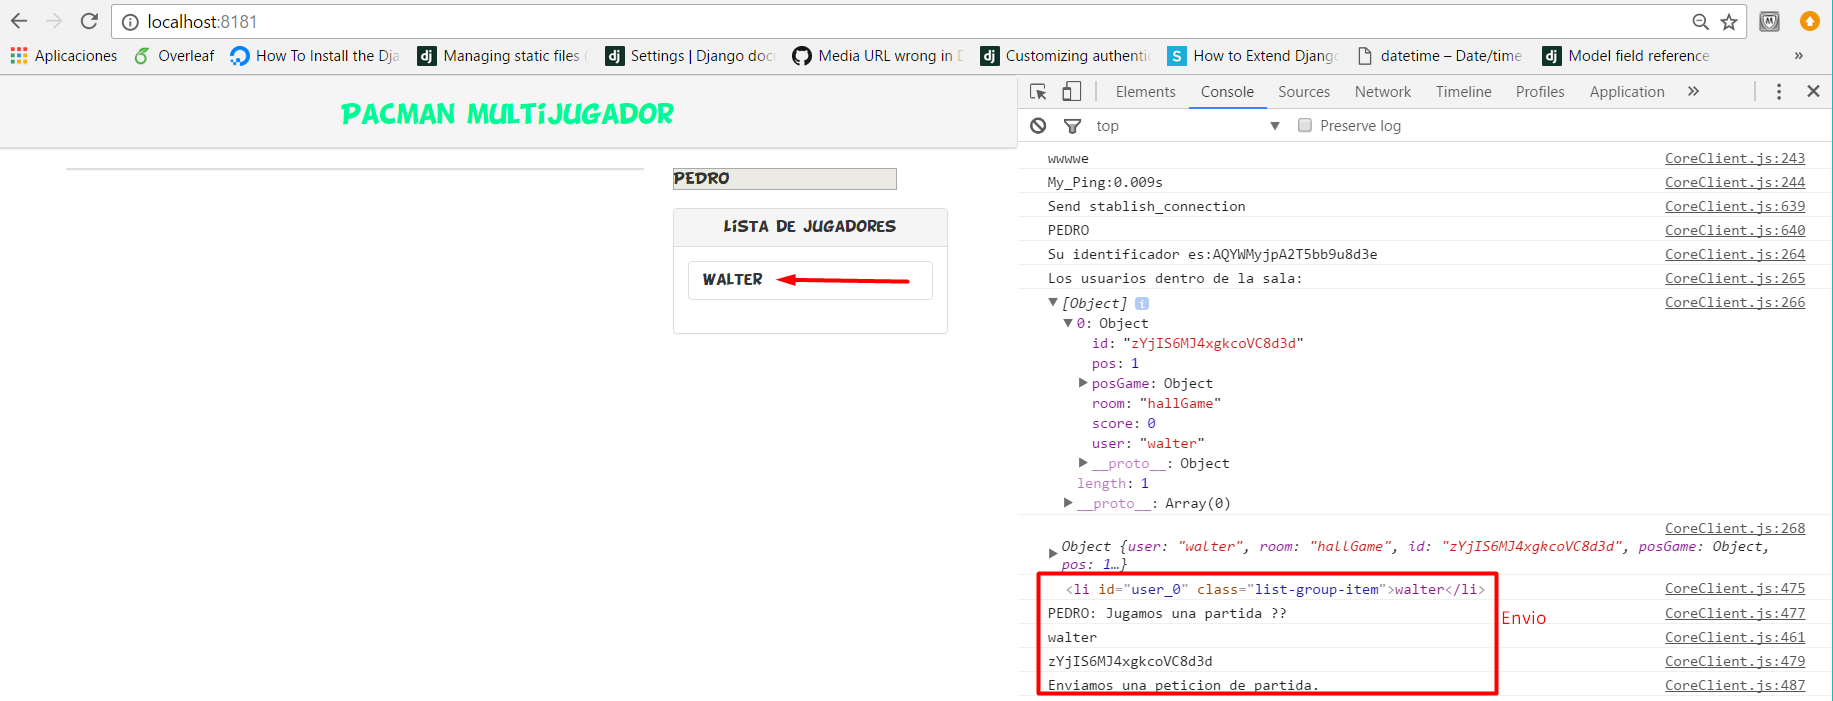
\includegraphics[width=0.8\linewidth]{Figures/Client2_Peti_Game}
	\decoRule
	\caption[Envió petición partida.]{Envió petición partida.}
\label{fig:Client2_Peti_Game}
\end{center}
\end{figure}
\\Los mensajes de petición de partida se crean entre usuarios por lo que el servidor solo nos sirve como intermediario para encaminar el mensaje. Por ello es necesario definir el evento \textbf{message} para gestionar estos mensajes.
\begin{lstlisting}[
caption=Definicion evento message.]
 socket.on('message',function(message){
  if(message.typeMsg == 'Init'){
   _message = message
   $('#peti').text(message.texto);
   $('#myModal').modal('show')
  }else if (message.typeMsg == 'replayInit') {
   if(message.texto == 'si'){
    $('#escena').show();
    CounterPacman = new Player(message.idOrigen);
    socket.emit('Request_ElementGame',CounterPacman.id);
   }else{
    $('li').on('click',function(){requestGame(this)});
   }
  }	
 });
\end{lstlisting}
Para el mensaje tipo \textbf{Init} el evento se encarga de mostrar una ventana emergente con la petición recibida, figura \ref{fig:Client1_Resep_Peti_Game}.
\begin{figure}[!h]
\begin{center}
   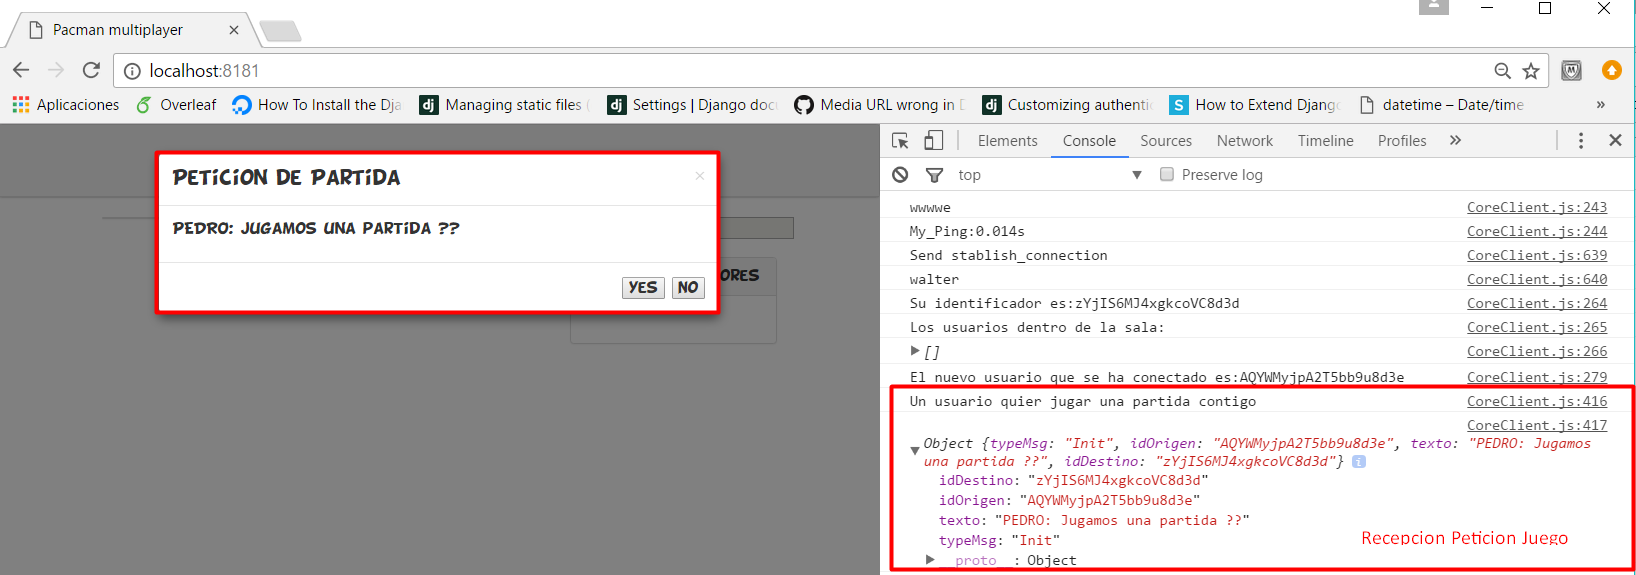
\includegraphics[width=0.8\linewidth]{Figures/Client1_Resep_Peti_Game}
	\decoRule
	\caption[Recepción petición partida.]{Recepción petición partida.}
\label{fig:Client1_Resep_Peti_Game}
\end{center}
\end{figure}
\\El usuario receptor tiene la opción de pulsar si o no provocando que la función \textbf{ReplayGame(si/no)} gestione la respuesta. La función independientemente de la opción genera un mensaje \textbf{message} que contiene el \textbf{id\_origen}, \textbf{id\_destino}, la respuesta a la petición y como subtipo de mensaje \textbf{Replay\_Init}.
\\Solo si la respuesta es afirmativa crea el mensaje \textbf{Request\_ElementGame} dirigido al servidor para pedir los parámetros iniciales del juego.
\begin{lstlisting}[
caption=Definición función replayGame.]
 function replayGame(contesta){
  $('#myModal').modal('hide')
  var message = {
   'typeMsg':'replayInit',
   'idOrigen':myPacman.id,
   'texto':contesta,
   'idDestino':_message.idOrigen
  };
  socket.emit('message',message)
  if(contesta == 'si'){
   $('#escena').show();
   CounterPacman = new Player(_message.idOrigen)
   socket.emit('Request_ElementGame',CounterPacman.id);
  }
 }
\end{lstlisting}
El usuario que envió el mensaje inicial recibe un mensaje \textbf{replayInit} para realizar las mismas tareas que el otro usuario, figura \ref{fig:Cliente1_Response_PetiGame}.
\begin{figure}[!h]
\begin{center}
   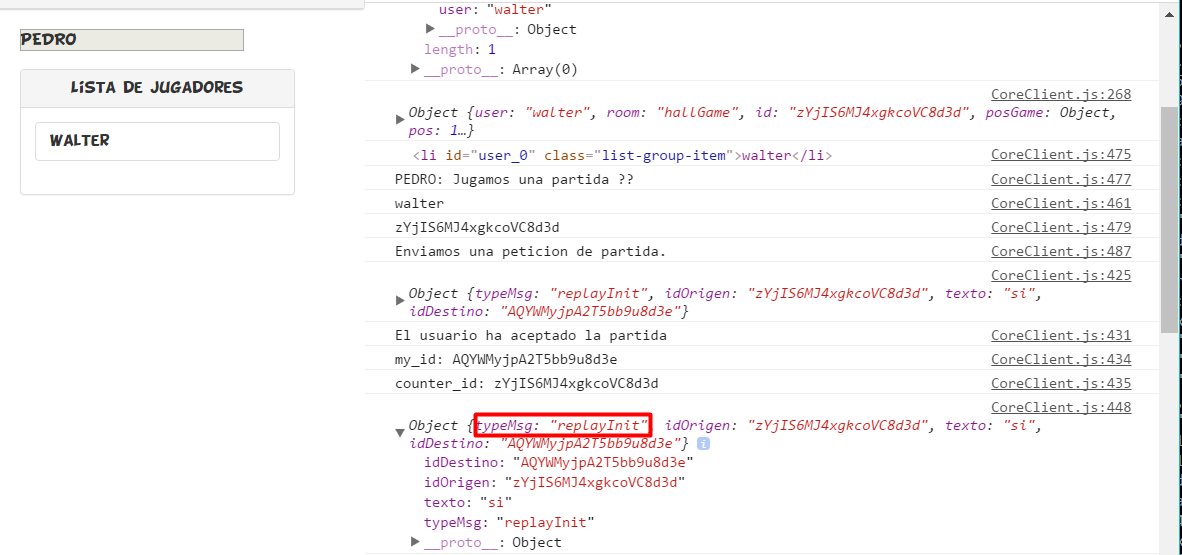
\includegraphics[width=0.8\linewidth]{Figures/Cliente1_Response_PetiGame}
	\decoRule
	\caption[Recepción respuesta a la petición de partida.]{Recepción respuesta a la petición de partida.}
\label{fig:Cliente1_Response_PetiGame}
\end{center}
\end{figure}
\subsubsection*{Presentación del juego}
Tras el ultimo mensaje enviado por los clientes es necesario definir el evento \textbf{Response\_ElementGame} para recibir el valor de los parámetros iniciales del juego.Los parámetros los obtiene de la variable \textbf{elements}, donde aquellos que tienen que ver con el escenario de juego se guardan en el objeto \textbf{GameArea} mientras que otros valores se guardan en \textbf{myPacman} y \textbf{CounterPacman} que corresponde al personaje del cliente y al del rival.
\begin{lstlisting}[
caption=Definicion evento Response\_ElementGame]
 socket.on('Response_ElementGame',function(elementsGame){
  GameArea.shape_1 = elementsGame.shape_1;
  GameArea.shape_2 = elementsGame.shape_2;
  GameArea.list_obstaculos=elementsGame.obstaculos;
  GameArea.list_cocos=elementsGame.cocos;
  GameArea.properGame=elementsGame.properGame;

  myPacman.setMyghostposition(elementsGame.myInfo.fantasma);
  delete elementsGame.myInfo.fantasma;
  myPacman.setMyPosition(elementsGame.myInfo);

  CounterPacman.setMyghostposition(elementsGame.counterInfo.fantasma);
  delete elementsGame.counterInfo.fantasma;
  CounterPacman.setMyPosition(elementsGame.counterInfo);
 
  DrawScene();
  socket.emit('Finish_InitFrame');
});
\end{lstlisting}
Con esta información llamamos a la función \textbf{Drawscene()} que define las dimensiones del área del juego y dibujar el aspecto inicial del juego a través de la función \textbf{UpdateGame()}.
\begin{lstlisting}[
caption=Definición función DrawScene.]
 function DrawScene(){
  GameArea.canvas.width=(GameArea.properGame.nFila+2)*GameArea.properGame.wCuad;
  GameArea.canvas.height=(GameArea.properGame.nColum+4)*GameArea.properGame.hCuad;
  $('#pnCanvas').show();
  UpdateGame();
}
\end{lstlisting}
La figura \ref{fig:Player1_frameInit} muestra la recepción de los parámetros y la visualización del juego para el primero usuario mientras la figura \ref{fig:Player2_frameInit} se muestra el del segundo usuario.
\begin{figure}[!h]
\begin{center}
   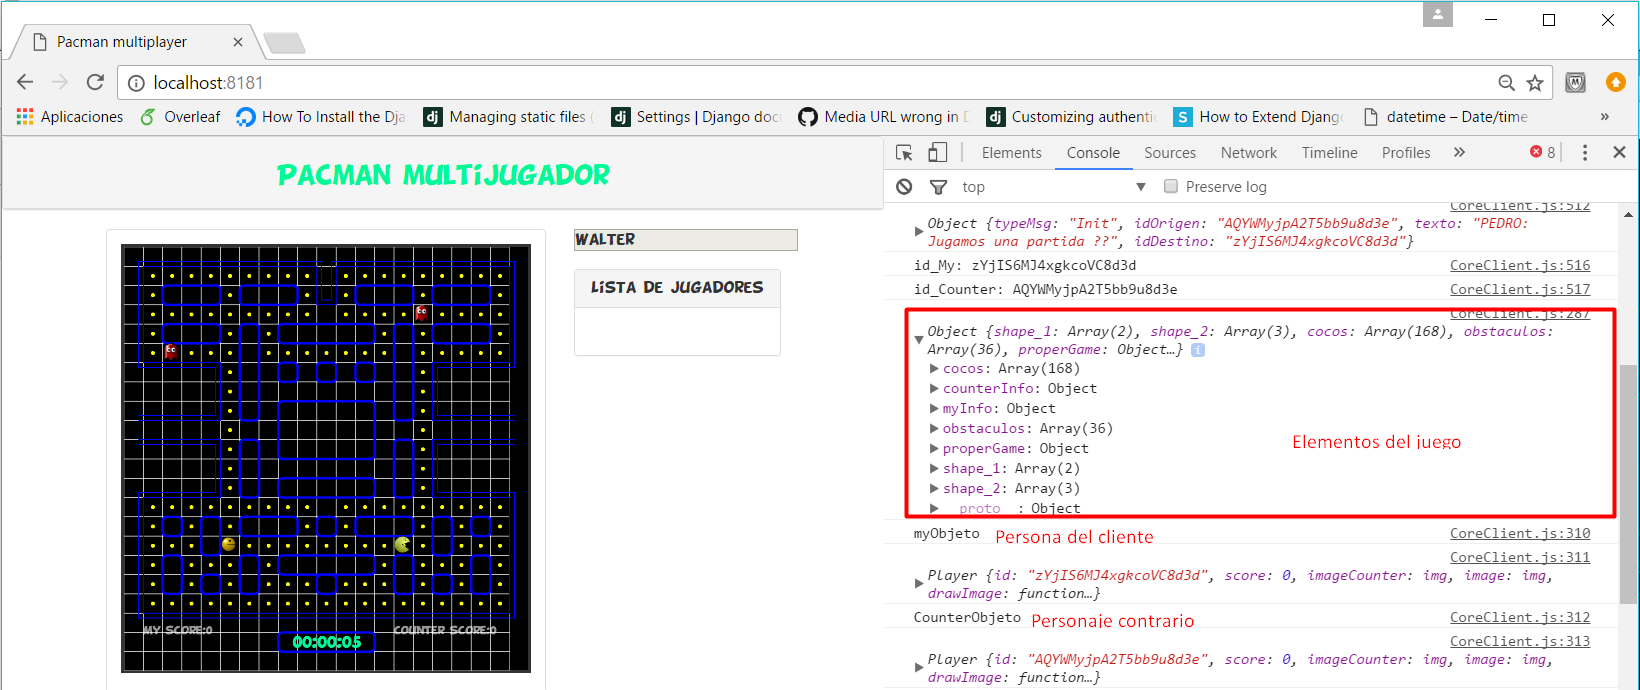
\includegraphics[width=0.8\linewidth]{Figures/Player1_frameInit}
	\decoRule
	\caption[Recepción parámetros iniciales 1ª usuario.]{Recepción parámetros iniciales 1ª usuario.}
\label{fig:Player1_frameInit}
\end{center}
\end{figure}
\begin{figure}[!h]
\begin{center}
   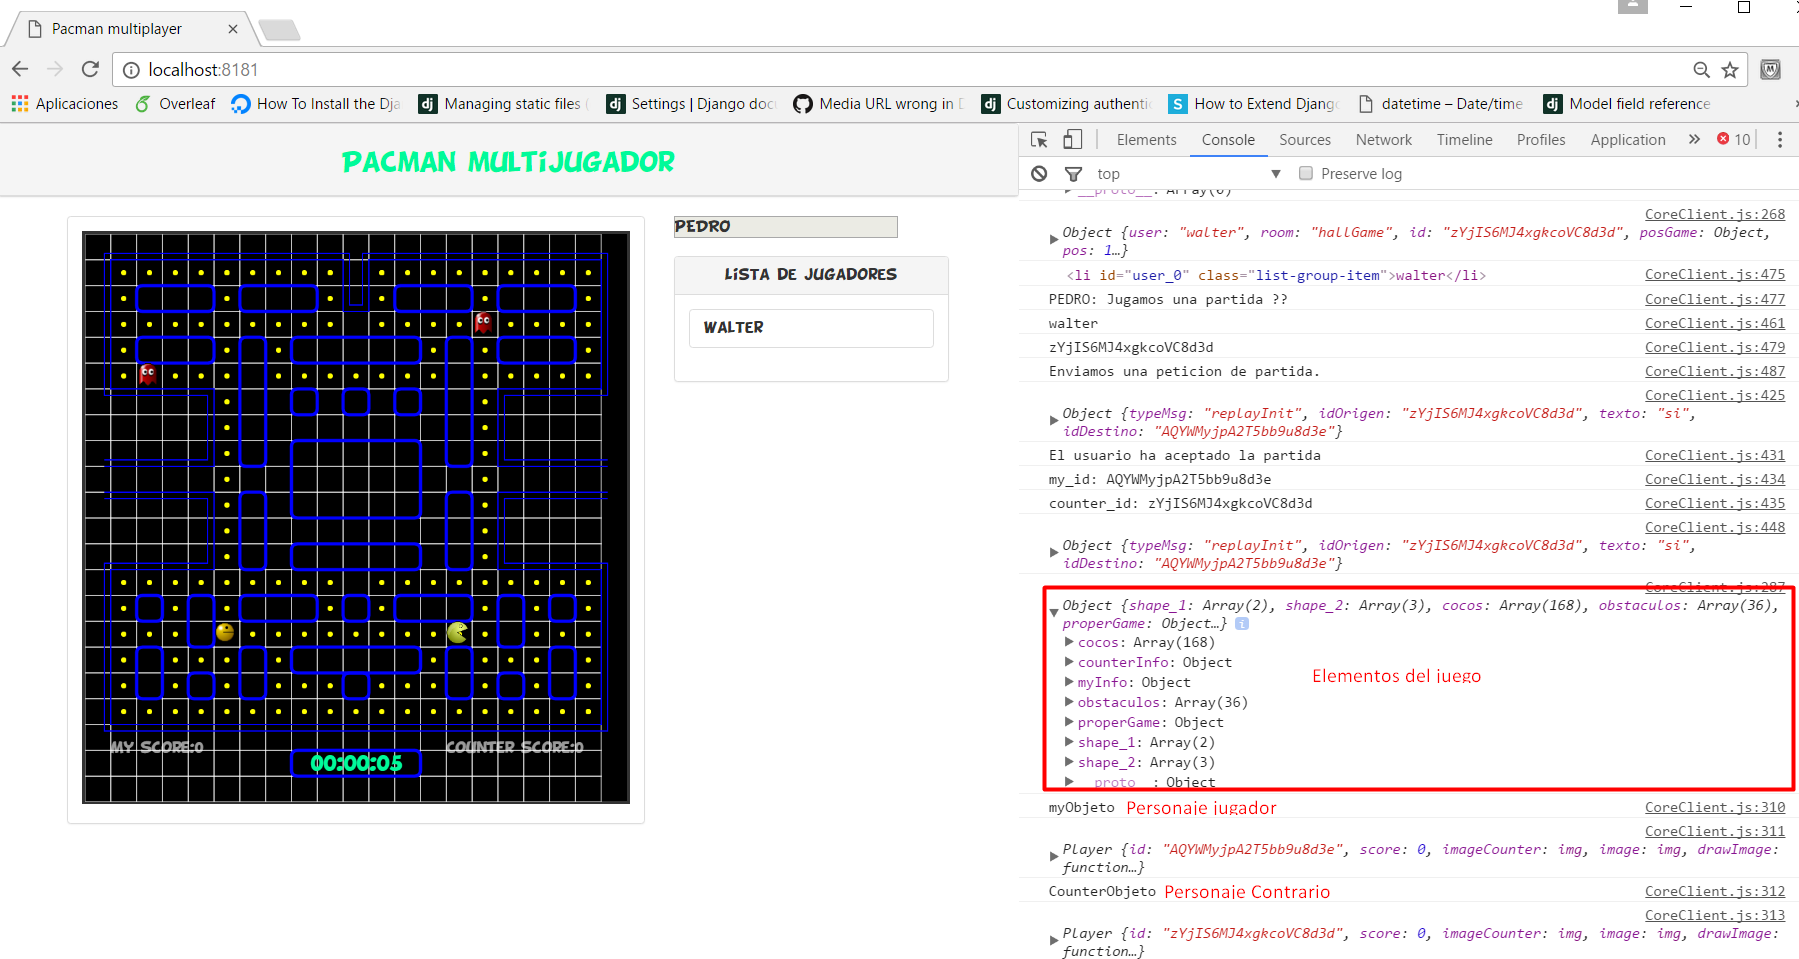
\includegraphics[width=0.8\linewidth]{Figures/Player2_frameInit}
	\decoRule
	\caption[Recepción parámetros iniciales 2ª usuario.]{Recepción parámetros iniciales 2ª usuario.}
\label{fig:Player2_frameInit}
\end{center}
\end{figure}
\\Tras realizar estas operaciones envía un mensaje \textbf{Finish\_initFrame} para indicar al servidor que el cliente esta a la espera de empezar la partida.
\subsubsection*{Inicio del juego}
Se crea el evento \textbf{ReadyGame} para recibir el mensaje de inicio de juego. En este momento se genera un evento timeInterval que ejecuta función \textbf{UpdateGame()} cada 1000/60 s provocando el inicio del juego.
\begin{lstlisting}[
caption=Definición evento ReadyGame.]
 socket.on('ReadyGame',function(){
  x = true;
  GameArea.frame = setInterval(UpdateGame,1000/60);
 });
\end{lstlisting}
\subsubsection*{Actualización del juego}
El movimiento del personaje se realiza por medio de la función \textbf{NextPosPacman} que gestiona los eventos del teclado. Cada movimiento tiene que ser validado ya que esta nueva posición se envía al servidor.
\\Primero verifica que la nueva posición del jugador,variable \textbf{newCoord}, no sobrepase el contorno del juego por medio de la función\textbf{ Game.hitt\_counter(newCoord)} igual que con los obstáculos a través de función \textbf{GameArea.hitObject(newCoord)}.
\\Si estas dos validaciones son correctas, envía un mensaje \textbf{UpdatePosition\_Player} con la nueva posición.
\begin{lstlisting}[
caption=Definición función NextPosPacman.]
 function NextPosPacman(e){
  var newCoord = {'x':0,'y':0};
  if(GameAcive){
   var pas = 0;
   newCoord.x = myPacman.myposition.x;
   newCoord.y = myPacman.myposition.y;
   if(e.code == 'ArrowDown'){
    newCoord.y += 0.5;
    pas += 0.5;
   }else if(e.code == 'ArrowUp'){
    newCoord.y += -0.5;
    pas += -0.5;
   }else if(e.code == 'ArrowRight'){
    newCoord.x += 0.5;
    pas += 0.5;
   }else if (e.code == 'ArrowLeft'){
    newCoord.x += -0.5;
    pas += -0.5;
   }
   var HitContor = GameArea.hitt_counter(newCoord);
   if(!HitContor){
    var HitObstacle = GameArea.hitObject(newCoord);
    if(!HitObstacle){
     myPacman.myposition.x = newCoord.x; 
     myPacman.myposition.y = newCoord.y;
     myPacman.myposition.numPasos += pas;
     socket.emit('UpdatePosition_Player',myPacman.myposition);
     if(myPacman.myposition.numPasos == 1 || myPacman.myposition.numPasos == -1){
      myPacman.myposition.numPasos = 0;
     }
     var eat = GameArea.eatCoco(myPacman.myposition);
     if(eat >= 0){
      socket.emit('UpdateCocos',eat);
     }
    }
   }
  }
 }
\end{lstlisting}
Ademas, comprueba si existe colisión con algún coco por medio de la función \textbf{GameArea.eatCoco(newCoord)}.En caso afirmativo envía un mensaje \textbf{UpdateCoco} con la posición del coco con el que se ha colisionado.
\\Las acciones anteriores las realizan los dos usuarios por lo que es necesario definir una serie de eventos para actualizar el estado del jugador contrario. 
\\El primer evento es \textbf{socket.on('NewPos\_Counter',function())} que recibe la nueva posición del usuario contrario.
\begin{lstlisting}[
caption=Definición evento NewPos\_Counter.]
 socket.on('NewPos_Counter',function(newPosition){
  CounterPacman.myposition = newPosition;
 });
\end{lstlisting}
El siguiente evento a definir es \textbf{socket.on('UpdateCocos\_Players',function())} que recibe la posicion del coco que ha comido el usuario contrario.
\begin{lstlisting}[
caption=Definición evento UpdateCocos\_Player.]
 socket.on('UpdateCocos_Player',function(cocoPosition){
  GameArea.list_cocos.splice(cocoPosition,1);
 });
\end{lstlisting}
Por ultimo se define el evento \textbf{socket.on(NewPos\_Ghost,function())} que recibe actualizaciones periódicas del servidor con la posición de los fantasmas, el valor del cronometro y la puntuación de cada usuario.
\begin{lstlisting}[
caption=Definición evento NewPos\_Ghost.]
 socket.on('NewPos_Ghost',function(fantasmas,timers,scores){
  GameArea.time = timers;
  for (var i = 0; i < fantasmas.length; i++) {
   ghost = fantasmas[i];
   core = scores[i];
   if(ghost.id == myPacman.id && core.id == myPacman.id){
    myPacman.myGhost.x = ghost.x;
    myPacman.myGhost.y = ghost.y;
    myPacman.score = core.score;			
   }else{
    CounterPacman.myGhost.x = ghost.x;
    CounterPacman.myGhost.y = ghost.y;
    CounterPacman.score = core.score;
   }
  }
 });
\end{lstlisting}
En las figuras \ref{fig:Update_Ghots_1}, \ref{fig:Update_Ghots_2} se muestra la recepción de los elementos del juego por cada usuario.
\begin{figure}[!h]
\begin{center}
   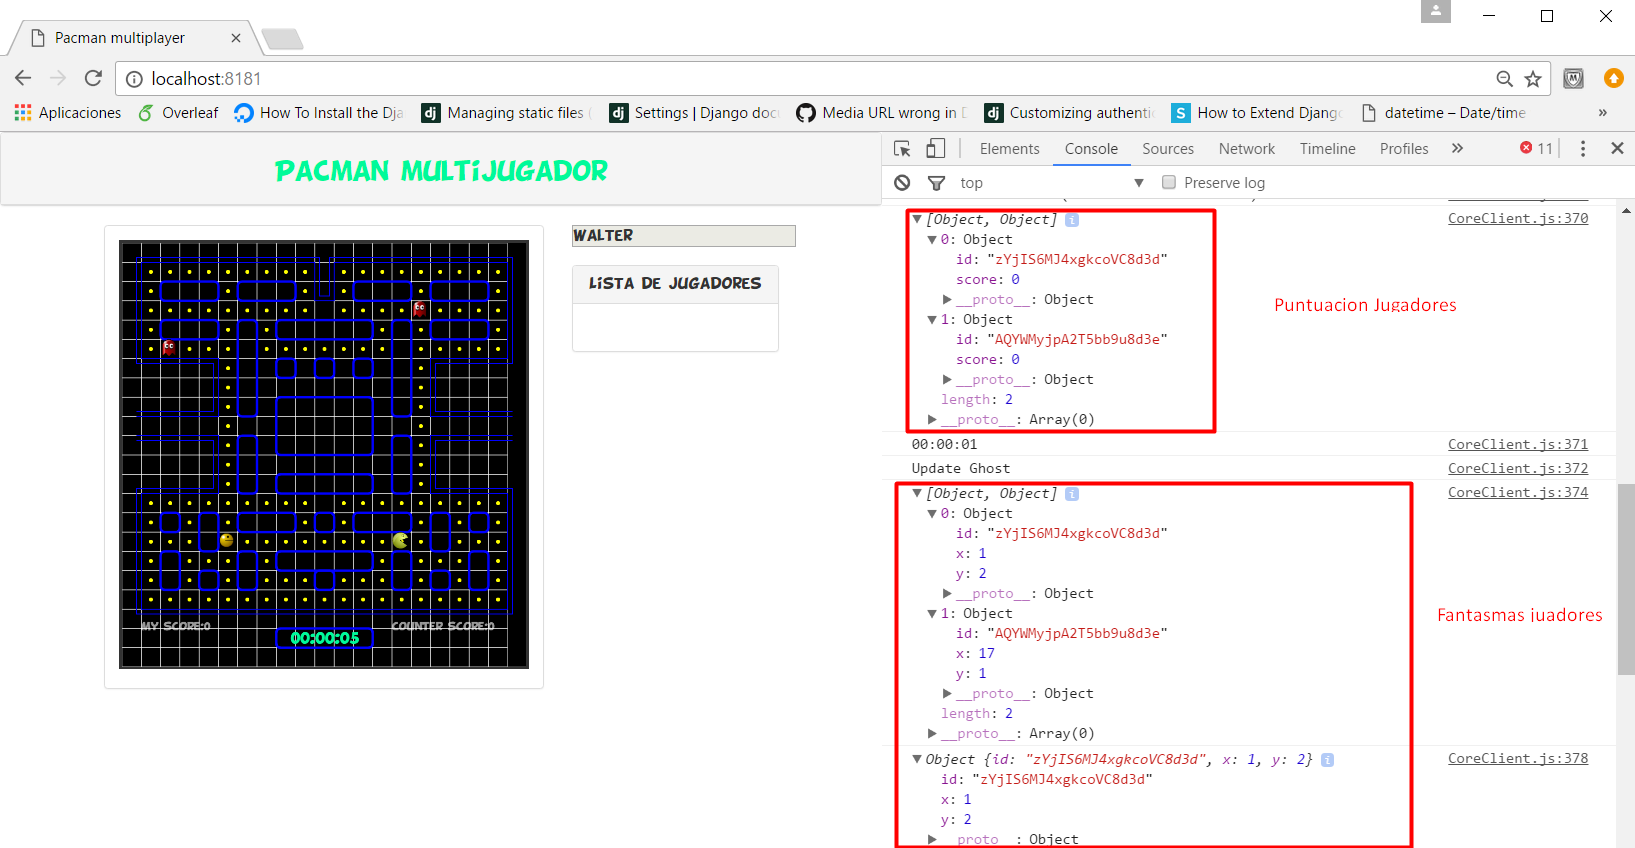
\includegraphics[width=0.6\linewidth]{Figures/Update_Ghots_1}
	\decoRule
	\caption[Recepción NewPos\_Ghost 1ª usuario.]{Recepción NewPos\_Ghost 1ª usuario.}
\label{fig:Update_Ghots_1}
\end{center}
\end{figure}
\begin{figure}[!h]
\begin{center}
   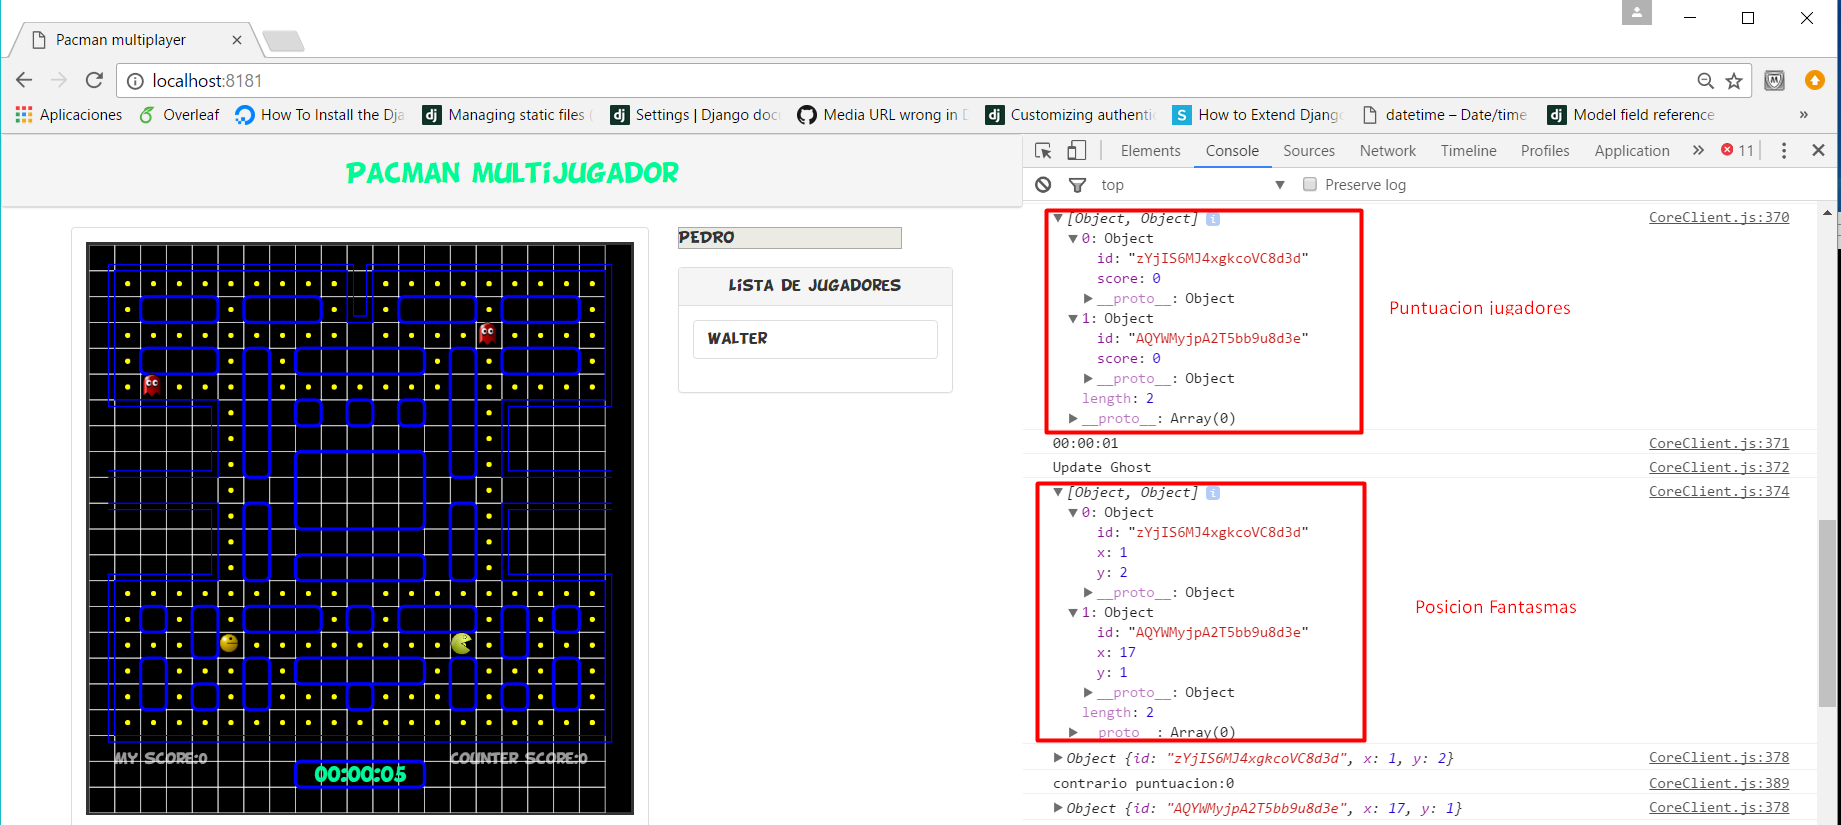
\includegraphics[width=0.6\linewidth]{Figures/Update_Ghots_2}
	\decoRule
	\caption[Recepción NewPos\_Ghost 2ª usuario.]{Recepción NewPos\_Ghost 2ª usuario.}
\label{fig:Update_Ghots_2}
\end{center}
\end{figure}
\subsubsection*{Finalización del juego}
Por ultimo, la finalización del juego lo determina el servidor ya que se encarga de comprobar si existe colisión con entre los jugadores y el fantasma.Por ello se define el evento \textbf{State\_Game} que recibe \textbf{OK} o \textbf{KO} dependiendo si jugador que ha sido capturado por el fantasma o no.
\begin{lstlisting}[
caption=Definición evento State\_Game.]
 socket.on('State_Game',function(msg){
  GameArea.State_Game = msg;
 });
\end{lstlisting}
La figura \ref{fig:Captura_Pacman} muestra como uno de los jugadores es capturado por el fantasma por lo que pierde la partida.
\begin{figure}[!h]
\begin{center}
   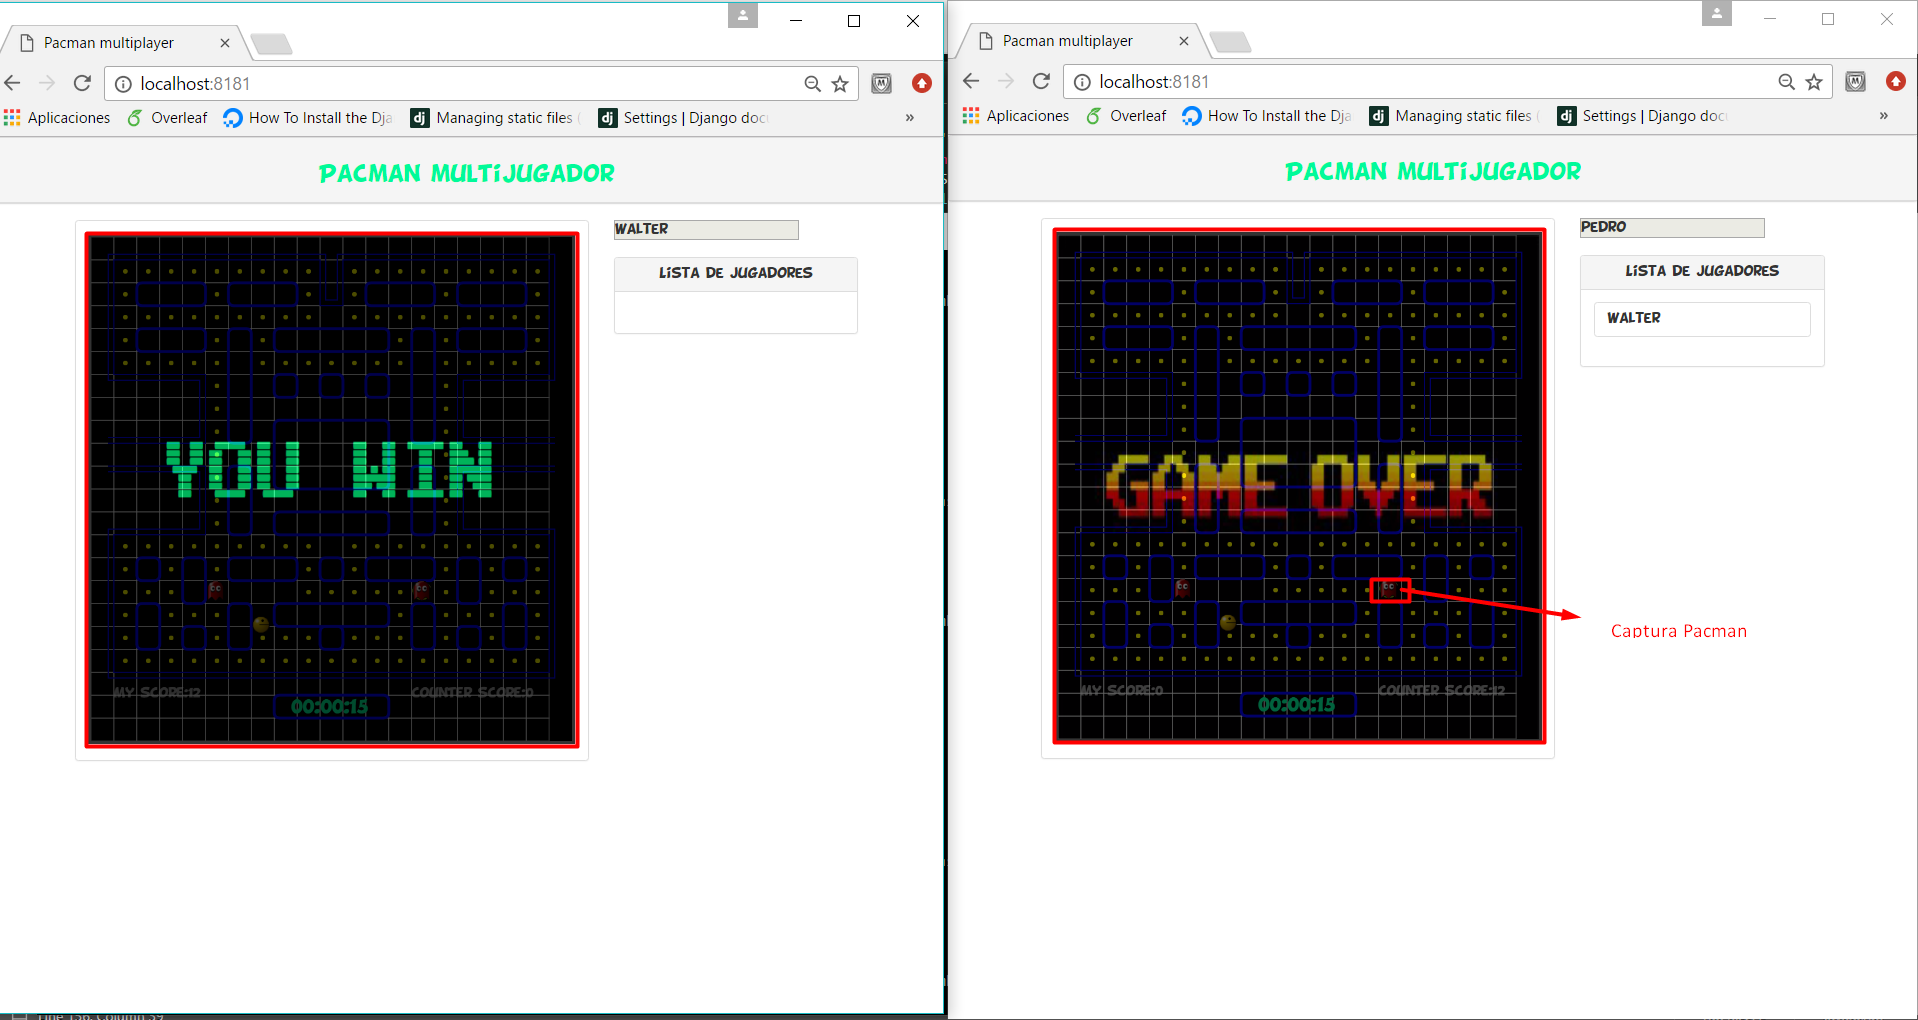
\includegraphics[width=0.6\linewidth]{Figures/Captura_Pacman}
	\decoRule
	\caption[Aspecto clásico Pacman]{Aspecto clásico Pacman.}
\label{fig:Captura_Pacman}
\end{center}
\end{figure}
\\Otro evento necesario es \textbf{GameWinner} que recibe el ganador de la partida cuando todos los cocos del coco han sido comidos.
\begin{lstlisting}[
caption=Definición evento GameWinner.]
 socket.on('GameWinner',function(userwiner){
  GameArea.State_Game = userwiner;
 });
\end{lstlisting}
\section{Pruebas}